% Created by tikzDevice version 0.12.3.1 on 2021-03-17 17:12:33
% !TEX encoding = UTF-8 Unicode
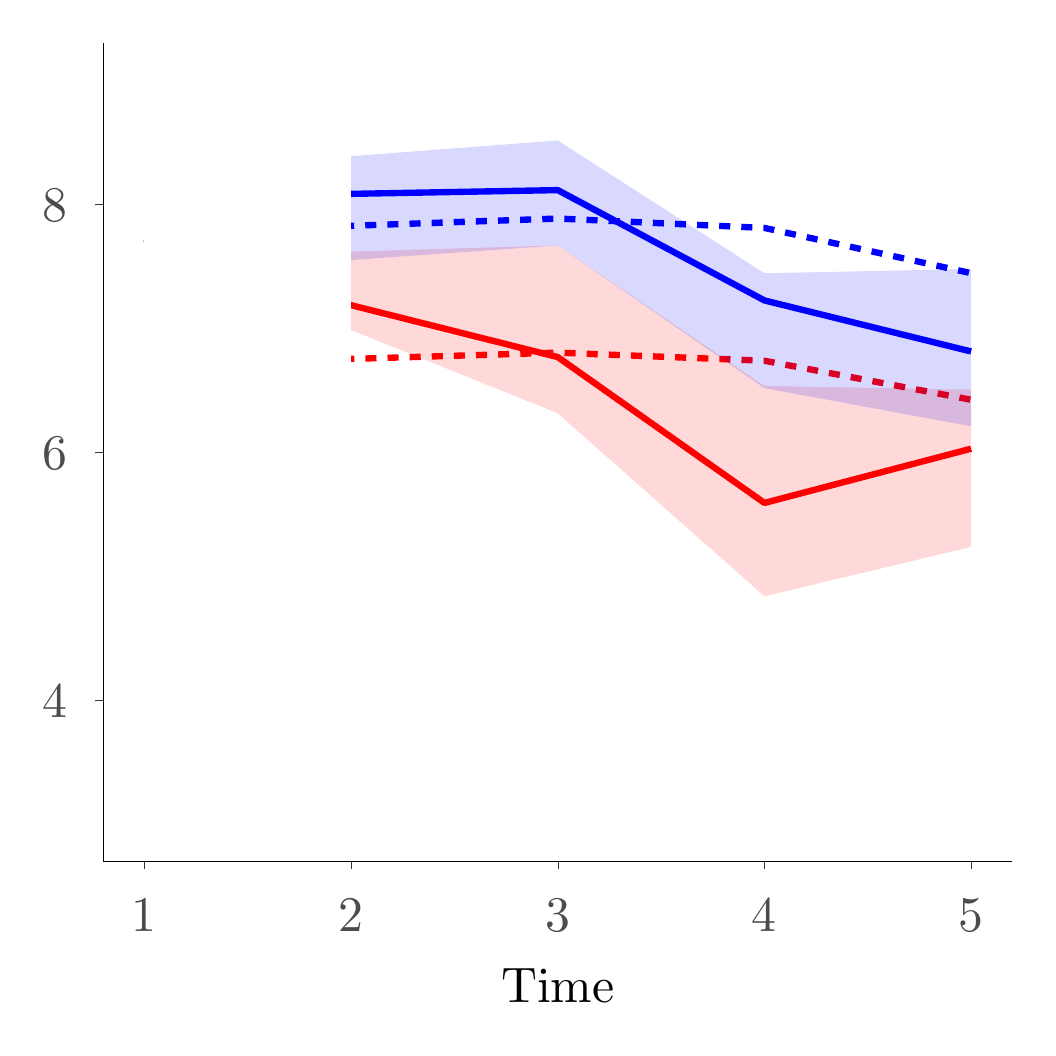
\begin{tikzpicture}[x=1pt,y=1pt]
\definecolor{fillColor}{RGB}{255,255,255}
\path[use as bounding box,fill=fillColor,fill opacity=0.00] (0,0) rectangle (361.35,361.35);
\begin{scope}
\path[clip] (  0.00,  0.00) rectangle (361.35,361.35);
\definecolor{drawColor}{RGB}{255,255,255}
\definecolor{fillColor}{RGB}{255,255,255}

\path[draw=drawColor,line width= 0.1pt,line join=round,line cap=round,fill=fillColor] (  0.00,  0.00) rectangle (361.35,361.35);
\end{scope}
\begin{scope}
\path[clip] ( 27.25, 60.04) rectangle (355.85,355.85);
\definecolor{fillColor}{RGB}{255,255,255}

\path[fill=fillColor] ( 27.25, 60.04) rectangle (355.85,355.85);
\definecolor{fillColor}{RGB}{255,0,0}

\path[fill=fillColor,fill opacity=0.15] ( 42.18,295.46) --
	(116.87,280.45) --
	(191.55,282.67) --
	(266.23,231.88) --
	(340.91,230.55) --
	(340.91,173.72) --
	(266.23,155.87) --
	(191.55,222.00) --
	(116.87,252.09) --
	( 42.18,251.33) --
	cycle;

\path[] ( 42.18,295.46) --
	(116.87,280.45) --
	(191.55,282.67) --
	(266.23,231.88) --
	(340.91,230.55);

\path[] (340.91,173.72) --
	(266.23,155.87) --
	(191.55,222.00) --
	(116.87,252.09) --
	( 42.18,251.33);
\definecolor{drawColor}{RGB}{255,0,0}

\path[draw=drawColor,line width= 2.3pt,line join=round] ( 42.18,285.12) --
	(116.87,261.07) --
	(191.55,242.31) --
	(266.23,189.61) --
	(340.91,209.21);

\path[draw=drawColor,line width= 2.3pt,dash pattern=on 4pt off 4pt ,line join=round] ( 42.18,236.91) --
	(116.87,241.65) --
	(191.55,243.92) --
	(266.23,240.99) --
	(340.91,226.89);
\definecolor{fillColor}{RGB}{0,0,255}

\path[fill=fillColor,fill opacity=0.15] ( 42.18,308.85) --
	(116.87,314.91) --
	(191.55,320.59) --
	(266.23,272.60) --
	(340.91,274.13) --
	(340.91,217.31) --
	(266.23,231.08) --
	(191.55,282.67) --
	(116.87,277.38) --
	( 42.18,271.18) --
	cycle;

\path[] ( 42.18,308.85) --
	(116.87,314.91) --
	(191.55,320.59) --
	(266.23,272.60) --
	(340.91,274.13);

\path[] (340.91,217.31) --
	(266.23,231.08) --
	(191.55,282.67) --
	(116.87,277.38) --
	( 42.18,271.18);
\definecolor{drawColor}{RGB}{0,0,255}

\path[draw=drawColor,line width= 2.3pt,line join=round] ( 42.18,293.08) --
	(116.87,301.29) --
	(191.55,302.65) --
	(266.23,262.78) --
	(340.91,244.34);

\path[draw=drawColor,line width= 2.3pt,dash pattern=on 4pt off 4pt ,line join=round] ( 42.18,284.26) --
	(116.87,289.75) --
	(191.55,292.38) --
	(266.23,288.98) --
	(340.91,272.64);
\definecolor{fillColor}{RGB}{255,255,255}

\path[fill=fillColor] ( 42.18, 60.04) rectangle (116.87,355.85);

\path[fill=fillColor] ( 42.18, 60.04) rectangle (116.87,355.85);

\path[fill=fillColor] ( 42.18, 60.04) rectangle (116.87,355.85);

\path[fill=fillColor] ( 42.18, 60.04) rectangle (116.87,355.85);

\path[fill=fillColor] ( 42.18, 60.04) rectangle (116.87,355.85);
\end{scope}
\begin{scope}
\path[clip] (  0.00,  0.00) rectangle (361.35,361.35);
\definecolor{drawColor}{RGB}{0,0,0}

\path[draw=drawColor,line width= 0.1pt,line join=round] ( 27.25, 60.04) --
	( 27.25,355.85);
\end{scope}
\begin{scope}
\path[clip] (  0.00,  0.00) rectangle (361.35,361.35);
\definecolor{drawColor}{gray}{0.30}

\node[text=drawColor,anchor=base east,inner sep=0pt, outer sep=0pt, scale=  1.80] at ( 14.50,112.11) {4};

\node[text=drawColor,anchor=base east,inner sep=0pt, outer sep=0pt, scale=  1.80] at ( 14.50,201.75) {6};

\node[text=drawColor,anchor=base east,inner sep=0pt, outer sep=0pt, scale=  1.80] at ( 14.50,291.39) {8};
\end{scope}
\begin{scope}
\path[clip] (  0.00,  0.00) rectangle (361.35,361.35);
\definecolor{drawColor}{gray}{0.20}

\path[draw=drawColor,line width= 0.1pt,line join=round] ( 24.50,118.31) --
	( 27.25,118.31);

\path[draw=drawColor,line width= 0.1pt,line join=round] ( 24.50,207.95) --
	( 27.25,207.95);

\path[draw=drawColor,line width= 0.1pt,line join=round] ( 24.50,297.58) --
	( 27.25,297.58);
\end{scope}
\begin{scope}
\path[clip] (  0.00,  0.00) rectangle (361.35,361.35);
\definecolor{drawColor}{RGB}{0,0,0}

\path[draw=drawColor,line width= 0.1pt,line join=round] ( 27.25, 60.04) --
	(355.85, 60.04);
\end{scope}
\begin{scope}
\path[clip] (  0.00,  0.00) rectangle (361.35,361.35);
\definecolor{drawColor}{gray}{0.20}

\path[draw=drawColor,line width= 0.1pt,line join=round] ( 42.18, 57.29) --
	( 42.18, 60.04);

\path[draw=drawColor,line width= 0.1pt,line join=round] (116.87, 57.29) --
	(116.87, 60.04);

\path[draw=drawColor,line width= 0.1pt,line join=round] (191.55, 57.29) --
	(191.55, 60.04);

\path[draw=drawColor,line width= 0.1pt,line join=round] (266.23, 57.29) --
	(266.23, 60.04);

\path[draw=drawColor,line width= 0.1pt,line join=round] (340.91, 57.29) --
	(340.91, 60.04);
\end{scope}
\begin{scope}
\path[clip] (  0.00,  0.00) rectangle (361.35,361.35);
\definecolor{drawColor}{gray}{0.30}

\node[text=drawColor,anchor=base,inner sep=0pt, outer sep=0pt, scale=  1.80] at ( 42.18, 34.90) {1};

\node[text=drawColor,anchor=base,inner sep=0pt, outer sep=0pt, scale=  1.80] at (116.87, 34.90) {2};

\node[text=drawColor,anchor=base,inner sep=0pt, outer sep=0pt, scale=  1.80] at (191.55, 34.90) {3};

\node[text=drawColor,anchor=base,inner sep=0pt, outer sep=0pt, scale=  1.80] at (266.23, 34.90) {4};

\node[text=drawColor,anchor=base,inner sep=0pt, outer sep=0pt, scale=  1.80] at (340.91, 34.90) {5};
\end{scope}
\begin{scope}
\path[clip] (  0.00,  0.00) rectangle (361.35,361.35);
\definecolor{drawColor}{RGB}{0,0,0}

\node[text=drawColor,anchor=base,inner sep=0pt, outer sep=0pt, scale=  1.80] at (191.55,  9.00) {Time};
\end{scope}
\end{tikzpicture}
